% Copyright 2004 by Till Tantau <tantau@users.sourceforge.net>.
%
% In principle, this file can be redistributed and/or modified under
% the terms of the GNU Public License, version 2.
%
% However, this file is supposed to be a template to be modified
% for your own needs. For this reason, if you use this file as a
% template and not specifically distribute it as part of a another
% package/program, I grant the extra permission to freely copy and
% modify this file as you see fit and even to delete this copyright
% notice. 

\documentclass{beamer}
\usepackage{graphicx}
\graphicspath{ {Images/} }
\usepackage{graphicx}
\usepackage{caption}
\usepackage{subcaption}
\usepackage{float}
\usepackage{biblatex}

\addbibresource{ref.bib}

\usepackage{tikz}
\usetikzlibrary{shapes.geometric, arrows}
\tikzstyle{startstop} = [rectangle, rounded corners, minimum width=3cm, minimum height=1cm,text centered, draw=black, fill=red!30]
\tikzstyle{io} = [trapezium, trapezium left angle=70, trapezium right angle=110, minimum width=3cm, minimum height=1cm, text centered, draw=black, fill=blue!30]
\tikzstyle{process} = [rectangle, minimum width=3cm, minimum height=1cm, text centered, draw=black, fill=orange!30]
\tikzstyle{decision} = [diamond, minimum width=3cm, minimum height=1cm, text centered, draw=black, fill=green!30]
\tikzstyle{arrow} = [thick,->,>=stealth]
\tikzstyle{Memory} = [cylinder,shape border rotate=90,draw,minimum height=2.5cm,minimum width=2cm]

% There are many different themes available for Beamer. A comprehensive
% list with examples is given here:
% http://deic.uab.es/~iblanes/beamer_gallery/index_by_theme.html
% You can uncomment the themes below if you would like to use a different
% one:
%\usetheme{AnnArbor}
%\usetheme{Antibes}
%\usetheme{Bergen}
%\usetheme{Berkeley}
%\usetheme{Berlin}
%\usetheme{Boadilla}
%\usetheme{boxes}
%\usetheme{CambridgeUS}
%\usetheme{Copenhagen}
%\usetheme{Darmstadt}
%\usetheme{default}
%\usetheme{Frankfurt}
%\usetheme{Goettingen}
%\usetheme{Hannover}
%\usetheme{Ilmenau}
%\usetheme{JuanLesPins}
%\usetheme{Luebeck}
\usetheme{Madrid}
%\usetheme{Malmoe}
%\usetheme{Marburg}
%\usetheme{Montpellier}
%\usetheme{PaloAlto}
%\usetheme{Pittsburgh}
%\usetheme{Rochester}
%\usetheme{Singapore}
%\usetheme{Szeged}
%\usetheme{Warsaw}

\title{Automated Evaluation of Programming Assignments}

% A subtitle is optional and this may be deleted
%\subtitle{}

\author{Rishabh Manoj}
% - Give the names in the same order as the appear in the paper.
% - Use the \inst{?} command only if the authors have different
%   affiliation.

\institute{International Institute of Information Technology - Bangalore}

\date{\today}
% - Either use conference name or its abbreviation.
% - Not really informative to the audience, more for people (including
%   yourself) who are reading the slides online

\subject{Program Analysis}
% This is only inserted into the PDF information catalog. Can be left
% out. 

% If you have a file called "university-logo-filename.xxx", where xxx
% is a graphic format that can be processed by latex or pdflatex,
% resp., then you can add a logo as follows:

% \pgfdeclareimage[height=0.5cm]{university-logo}{university-logo-filename}
% \logo{\pgfuseimage{university-logo}}

% Delete this, if you do not want the table of contents to pop up at
% the beginning of each subsection:
\AtBeginSubsection[]
{
  \begin{frame}<beamer>{Outline}
    \tableofcontents[currentsection,currentsubsection]
  \end{frame}
}

% Let's get started
\begin{document}

\begin{frame}
  \titlepage
\end{frame}


% Section and subsections will appear in the presentation overview
% and table of contents.


\begin{frame}{Problem Statement}{}
    \begin{itemize}
        \item Automate the grading of programming solutions given a reference solution to a programming problem.\\
        \item Grades based on "correctness" measures of incorrect solutions.
    \end{itemize}
    
    
\end{frame}

\begin{frame}{Proposed Methods}{}
  \begin{itemize}
      \item \textbf{Gold Standard Solutions}: Separate given solns into \textit{correct} and \textit{incorrect} groups based on test-cases generated from reference solns. 
      \item \textbf{Similarity Measure}: Calculate the similarity measure of the correct solns with each other.
      \item \textbf{Clustering}: A fully connected graph can be constructed if each soln is considered as a node and the similarity measure value it's edge weight. Cluster this graph. Expected output is clusters of solutions with similar approaches.
      \item \textbf{Marking}: Calculate similarity measures of every incorrect solns to a representative solns of each of the clusters. Assign grades based on the "closeness" to cluster.  
  \end{itemize}
  
\end{frame}

\begin{frame}{Model Architecture}

\begin{center}

 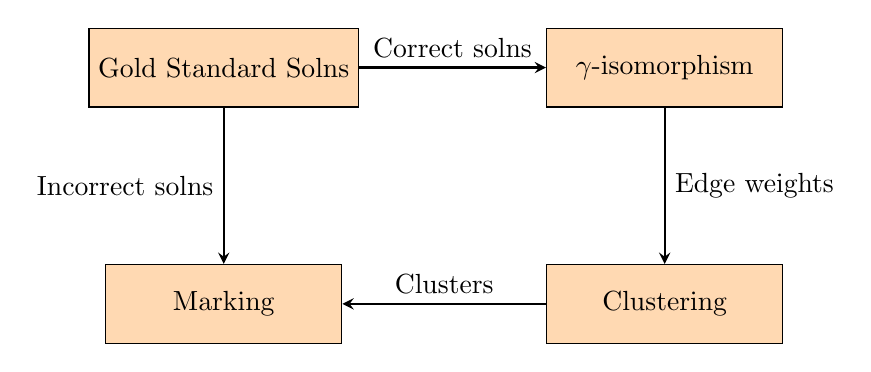
\begin{tikzpicture}[node distance=1.5cm]
   \node (pro1) [process] {Gold Standard Solns};
   \node (pro2) [process, right of=pro1, xshift = 4.1cm] {$\gamma$-isomorphism};
   \node (pro3) [process, below of=pro2, yshift = -1.5cm] {Clustering};
   \node (pro4) [process, left of=pro3, xshift = -4.1cm] {Marking};
   
   \draw [arrow] (pro1) -- node[anchor=south] {Correct solns} (pro2);
   \draw [arrow] (pro2) -- node[anchor=west] {Edge weights} (pro3);
   \draw [arrow] (pro3) -- node[anchor=south] {Clusters} (pro4);
    \draw [arrow] (pro1) -- node[anchor=east] {Incorrect solns} (pro4);
 \end{tikzpicture}    

\end{center}

\end{frame}

\begin{frame}{Similarity Measure}{Definitions}
    \begin{enumerate}
        \item \textbf{Data dependency:} A data dependency is a situation in which a program statement refers to the data of a preceding statement.\\
        \item \textbf{Control dependency:} Control dependency is a situation in which a program instruction executes if the previous instruction evaluates in a way that allows its execution. (\textit{if} statements, \textit{while} $\cdots$)\\
        \item \textbf{Isomorphism:} A graph can exist in different forms having the same number of vertices,edges and
also having same edge connectivity. Such graphs are called isomorphic graphs.\\
    \end{enumerate}
    
\end{frame}

\begin{frame}{Similarity Measure}{Definitions}
    \textbf{Program Dependence Graph:}\\ Program dependence graph (PDG) is a graphical representation of the source code of a program. Basic statements, like variable declarations, assignments, and procedure calls, are represented by program vertices in PDG’s. The data and control
dependencies between statements are represented by edges between program vertices
in PDG’s.\\

\end{frame}

\begin{frame}{Similarity Measure}
\begin{itemize}
    \item[] \textbf{$\gamma$-isomorphism:}\cite{Liu:2006:GDS:1150402.1150522}\\ 
   The central idea is to generate \textit{Program Dependence Graphs} for the solutions and check for sub-graph isomorphism between any two PDG's.\\
   If it is sub-graph isomorphic then based on the number of vertices mapped we calculate similarity.\\
    
    \textit{\textbf{Algorithm:}}
    \begin{itemize}
    \item Generate PDG's of the solution.
    \item Use $\gamma$-isomorphism method to calculate similarity between PDG's of all correct solutions. 
    \begin{itemize}
        \item This $\gamma$-isomorphism method checks for sub-graph isomorphism between the PDG's and calculates similarity measure.  
    \end{itemize}
    
    \end{itemize} 
\end{itemize}

\end{frame}

\begin{frame}{Similarity Measure}{Implementation}
    \begin{itemize}
        \item For each program, PDG has to be generated, we use \textit{frama-c} to generate a DOT file which contains the PDG.
        \item A DOTParser for python was used to extract nodes and edges from the DOT file. This was converted to a NetworkX graph in python.
        \item Sub graph isomorphism algorithm was used to calculate similarity.
    \end{itemize}
\end{frame}

\begin{frame}{Similarity Measure}{Implementation}
    \textbf{Program Dependence Graph}
        \begin{itemize}
            \item \textit{Frama-c} is a set of interoperable program analyzers for C programs. We use \textit{Frama-c} to generate dependency graph in the form of DOT files for C programs. While it generates for most of the C programs it does not encompass the entire C language. 
            \item The output of Frama-c's pdg generation is a DOT file which contains the nodes and edges of the PDG. DOT files are hard to interpret and contains unnecessary details, so a DOTParser was used to get only the nodes and edges. This was then used to instantiate a NetworkX graph (a python library for graphs) which was selected for it's vast graph related library.
        \end{itemize}
\end{frame}

\begin{frame}{Similarity Measure}{Implementation}
    \textbf{$\gamma$-isomorphism}
    \begin{itemize}
        \item We follow the algorithm provided in \cite{Liu:2006:GDS:1150402.1150522} named $\gamma$-isomorphism as it used a $\gamma$-filtering technique to eliminate certain graphs before performing subgraph isomorphism.
        
        \item  Sub graph Isomorphism is an NP-Complete problem which means that there is no polynomial time solution. (Note that Graph Isomorphism is neither P nor NP-complete but it's generalisation(sub-graph isomorphism) is NP-complete). Over the years there have been many heuristic solutions that attempt to solve this for a specific set of graphs like the Glasgow algorithm[\cite{Glasgow}], the VF2 algorithm[\cite{VFLib}] and recently the LAD filtering algorithm[\cite{pathLAD}].
    \end{itemize}
\end{frame}

\begin{frame}{Similarity Measure}{Implementation}
    \begin{itemize}
        \item Initially the \textit{VF2} algorithm was implemented as it was used in the algorithm mentioned in \cite{Liu:2006:GDS:1150402.1150522}, we found that the algorithm is very time-consuming, while for graphs with very less nodes (in the range of 20 to 30) it calculates in seconds, the higher the vertex count (usually in the range of 100's which is the case for our dataset) it sometimes takes days to calculate!!
        
        \item  Due to this the \textit{VF2} algorithm approach was abandoned and the latest development in sub graph isomorphism the LAD filtering approach was chosen due to it being the latest publications. The new variant, \textit{pathLAD} \cite{pathLAD}, was used. A time limit was set which can act as a threshold as to when the search can be discontinued.
    \end{itemize}
\end{frame}  

\begin{frame}{Similarity Measure}{Implementation}
    \begin{itemize}
        \item While the LAD algorithm works much faster than \textit{VF2}, there are still cases where sub-graphs could not be found within the time-limit. In some cases increasing the time-limit by a few seconds leads to solutions where it would not have found in the decreased time-space. This leads to drastic change in the output of the next phase. There are also cases where LAD filtering fails completely as the conditions required for the filtering are not met.
        
        \item  To overcome this, a plethora of subgraph isomorphism algortihm was used in conjunction with each other. The idea is that even if the conditions are not met for one algorithm then the other can pick up the slack.
    \end{itemize}
\end{frame}

\begin{frame}{Similarity Measure}{Visualisation}
     \begin{figure}[H]
            \centering
            \includegraphics[height=1.7in]{similarity_ensemble_old_frama_1.png}
            \caption*{Similarity Measurement Graph for a particular set of program files}
     \end{figure}
\end{frame}
\begin{frame}{Similarity Measure}{Visualisation}
     \begin{figure}
         \centering
         \includegraphics[height=1.7in]{similarity_ensemble_1.png}
         \caption*{Similarity Measurement Graph for a particular set of program files}
         \label{fig:my_label}
     \end{figure}
\end{frame}

\begin{frame}{Clustering}
\begin{itemize}
    \item Graph clustering involves the task of dividing nodes into clusters, so that the edge density is higher within clusters as opposed to across clusters.
    \item In this module we cluster similar solutions together to form some distinct types/methods/algorithms of solutions possible for the given problem.
    \item The output from the above Similarity Measure module is considered as an edgelist in this module. The program files become the nodes and the similarity measure becomes the weights of the edge between them.
    \item Using this graph, we start clustering. Idea is that nodes with edges whose similarity values are high will cluster together. 

    \item The output of this module are clusters which contains program files.
\end{itemize}

\end{frame}

\begin{frame}{Clustering}{Implementation Details}
We use various clustering algorithms and compare their clusters to some human annotated clusters.

    \textbf{Louvain modularity:}\\
    \begin{itemize}
        \item We use a method called Louvain modularity \cite{louvian} which is a greedy optimization method that appears to run in time O($n\log n$).
        \item In this method, first small communities are found by optimizing modularity locally on all nodes, then each small community is grouped into one node and the step is repeated.
    \end{itemize}
         
\end{frame}

\begin{frame}{Clustering}{Implementation Details}
    \begin{itemize}
        \item \textit{Observation:} Nodes within Clusters sometimes do not have high edge weights, while one node will be highly connected to everything the other nodes are not so strongly connected to each other node. \\ 
        \item \textit{Possible explanation:} Since similarity values are calculated based on isomorphism which is NP-complete, the values for some pair of nodes might actually be high but since it cannot be found out in the stipulated time interval, the values are given zero. While clustering, if the neighbours of the nodes are highly similar then it is also highly likely that the node is similar to the rest of the others.
        \item \textit{Solution:} Add other parameters to include in similarity measurement.
    \end{itemize}
\end{frame}

\begin{frame}{Clustering}{Implementation Details}

    \textbf{IPCA Clustering}\\
    \begin{itemize}
        \item Each point’s measure property can be transformed as the influence power against its neighbor points. If one point’s measure is larger, it would have more
influence power to attract its neighbor points, and its neighbors would have a trend to be absorbed by this point.
        \item  \textit{Observation:} Within clusters, the similarity is high but same nodes are found in multiple clusters
    \end{itemize}
\end{frame}

\begin{frame}{Clustering}{Visualisation}
     \begin{figure}[H]
            \centering
            \includegraphics[height=1.7in]{cluster_louvian_1.png}
            \caption*{Louvian Graph Clusters for a particular set of program files}
     \end{figure}
\end{frame}
\begin{frame}{Clustering}{Visualisation}
     \begin{figure}
         \centering
         \includegraphics[height=1.7in]{cluster_IPCA_1.png}
         \caption*{IPCA Graph Clusters for a particular set of program files}
     \end{figure}
\end{frame}

\begin{frame}{Clustering}{Visualisation}
     \begin{figure}[H]
            \centering
            \includegraphics[height=1.7in]{cluster_louvian_old_frama_1.png}
            \caption*{Louvian Graph Clusters for a particular set of program files}
     \end{figure}
\end{frame}
\begin{frame}{Clustering}{Visualisation}
     \begin{figure}
         \centering
         \includegraphics[height=1.7in]{cluster_IPCA_old_frama_1.png}
         \caption*{IPCA Graph Clusters for a particular set of program files}
     \end{figure}
\end{frame}

\begin{frame}{Marking}
     \begin{itemize}
         \item  This module is primarily for Incorrect solutions. The idea is to categorize the solution into the nearest cluster by calculating similarity measure with each of the Gold Standard solutions (Correct Solutions) and clustering into the nearest group.
    
        \item We get the similarity measure from the above module and find the most similar gold standard program and assign the cluster which the gold standard program is in.
    
        \item To assign a grade we use many factors like the no. of testcases it passed, the running time, amount of memory used, strength of similarity and intra-cluster distance, etc...
     \end{itemize}
\end{frame}

\begin{frame}{Marking}{Implementation}
     \begin{itemize}
         \item  Generate PDG's of incorrect solutions using the procedure described in Similarity Measure phase
         \item   Assign clusters to solutions based on similarity measured to a set representative of cluster and solution from Similarity Measure phase. (Set representative can be node with highest degree)
         \item  Train a regression model to assign grades
     \end{itemize}
\end{frame}



\begin{frame}{References:}
    
\printbibliography

\end{frame}
\end{document}


